\begin{abstract}

Here we define paradata as the data that describes the generation of data.
In genetic epidemiology, the data generated is mostly the results 
of an analysis (e.g. predicting a person having a disease),
as done by computer code.
In such context, paradata is usually the scientific paper that
describes what the computer code does.
However, this has the unrealtistic 
assumption that there is a perfect match between the paper and the code.
In this chapter it is argued that the source code should should be supplied,
as this is the true paradata: if the paper and code disagree, it is the
code that has generated the results.
The chapter concludes by some rules how to allow code to serve as paradata,
and hence allowing computational research to be truly reproducible.

\end{abstract}

{\bf Keywords:} paradata, reproducible research, code, software,
FAIR data, computational research, Open Science, DevOps, best practices,
genetic epidemiology

%%%%%%%%%%%%%%%%%%%%%%%%%%%%%%%%%%%%%%%%%%%%%%%%%%%%%%%%%%%%%%%%%%%%%%%%%%%%%%%%
\section*{Abbreviations}
%%%%%%%%%%%%%%%%%%%%%%%%%%%%%%%%%%%%%%%%%%%%%%%%%%%%%%%%%%%%%%%%%%%%%%%%%%%%%%%%

\begin{table}[h]
  \begin{tabular}{ll}
    Abbreviation & Full                                    \\
    \hline
    AI           & Artificial intelligence                 \\
    GCAE         & Genotype convolutional autoencoder      \\
    GWAS         & Genome-wide association study           \\
    ML           & Machine learning                        \\
    PCA          & Principal Component Analysis
  \end{tabular}
\end{table}

%%%%%%%%%%%%%%%%%%%%%%%%%%%%%%%%%%%%%%%%%%%%%%%%%%%%%%%%%%%%%%%%%%%%%%%%%%%%%%%%
\section{Introduction}
%%%%%%%%%%%%%%%%%%%%%%%%%%%%%%%%%%%%%%%%%%%%%%%%%%%%%%%%%%%%%%%%%%%%%%%%%%%%%%%%

\begin{figure}[!htbp]
  \centering
  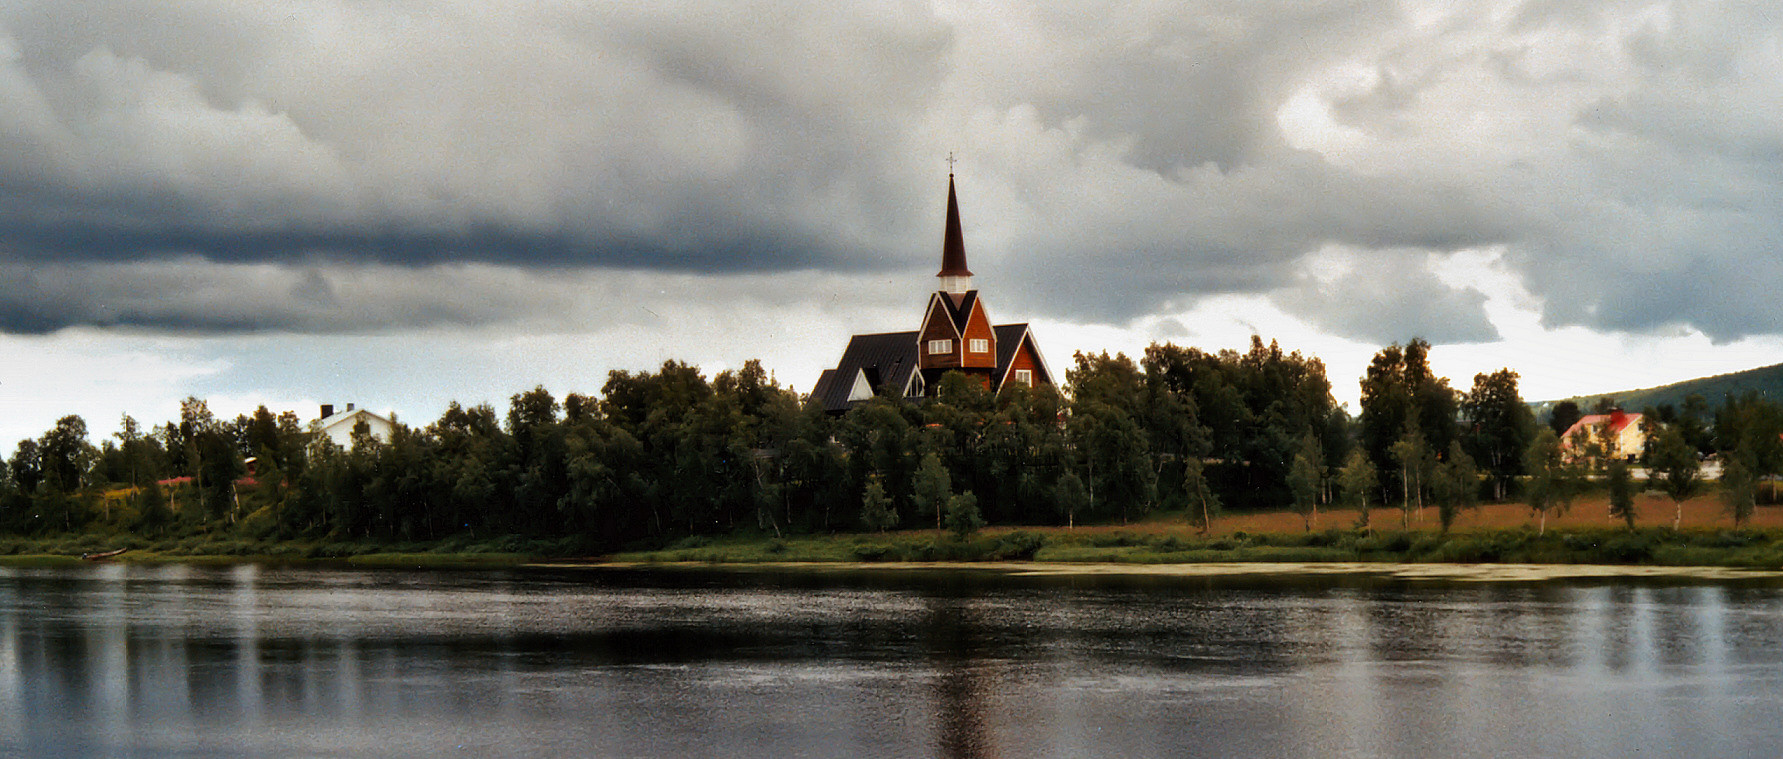
\includegraphics[width=\linewidth]{Karesuando_church.jpg}
  \caption{Karesuando's church}
  \label{fig:karesuando_church}
\end{figure}

%%%%%%%%%%%%%%%%%%%%%%%%%%%%%%%%%%%%%%%%%%%%%%%%%%%%%%%%%%%%%%%%%%%%%%%%%%%
\section{Discussion}
%%%%%%%%%%%%%%%%%%%%%%%%%%%%%%%%%%%%%%%%%%%%%%%%%%%%%%%%%%%%%%%%%%%%%%%%%%%

We found ...

%%%%%%%%%%%%%%%%%%%%%%%%%%%%%%%%%%%%%%%%%%%%%%%%%%%%%%%%%%%%%%%%%%%%%%%%%%%%%%%%
\section{Data Accessibility}
%%%%%%%%%%%%%%%%%%%%%%%%%%%%%%%%%%%%%%%%%%%%%%%%%%%%%%%%%%%%%%%%%%%%%%%%%%%%%%%%

This article and its metadata can be found at 
\url{https://github.com/richelbilderbeek/chapter_paradata}.

%%%%%%%%%%%%%%%%%%%%%%%%%%%%%%%%%%%%%%%%%%%%%%%%%%%%%%%%%%%%%%%%%%%%%%%%%%%%%%%%
% Bibliography
%%%%%%%%%%%%%%%%%%%%%%%%%%%%%%%%%%%%%%%%%%%%%%%%%%%%%%%%%%%%%%%%%%%%%%%%%%%%%%%%
% Vancouver style
\bibliographystyle{unsrtnat}
\bibliography{article}
%%%%%%%%%%%%%%%%%%%%%%%%%%%%%%%%%%%%%%%%%%%%%%%%%%%%%%%%%%%%%%%%%%%%%%%%%%%%%%%%

%%%%%%%%%%%%%%%%%%%%%%%%%%%%%%%%%%%%%%%%%%%%%%%%%%%%%%%%%%%%%%%%%%%%%%%%%%%%%
\newpage
\appendix
\section{Supplementary materials}

% Figures start from one and are prepended with an S
\renewcommand{\thefigure}{S\arabic{figure}}
\setcounter{figure}{0}

% Tables start from one and are prepended with an S
\renewcommand{\thetable}{S\arabic{table}}
\setcounter{table}{0}
%%%%%%%%%%%%%%%%%%%%%%%%%%%%%%%%%%%%%%%%%%%%%%%%%%%%%%%%%%%%%%%%%%%%%%%%%%%%%

%%%%%%%%%%%%%%%%%%%%%%%%%%%%%%%%%%%%%%%%%%%%%%%%%%%%%%%%%%%%%%%%%%%%%%%%%%%%%
\subsection{Datasets}
%%%%%%%%%%%%%%%%%%%%%%%%%%%%%%%%%%%%%%%%%%%%%%%%%%%%%%%%%%%%%%%%%%%%%%%%%%%%%

Stuff

